\chapter{Literature Review and Related Work}
\label{chap:relatedworks}

\section{Competitor Analysis}
\label{section:competitor-analysis}

\begin{figure}[ht]
    \centering
    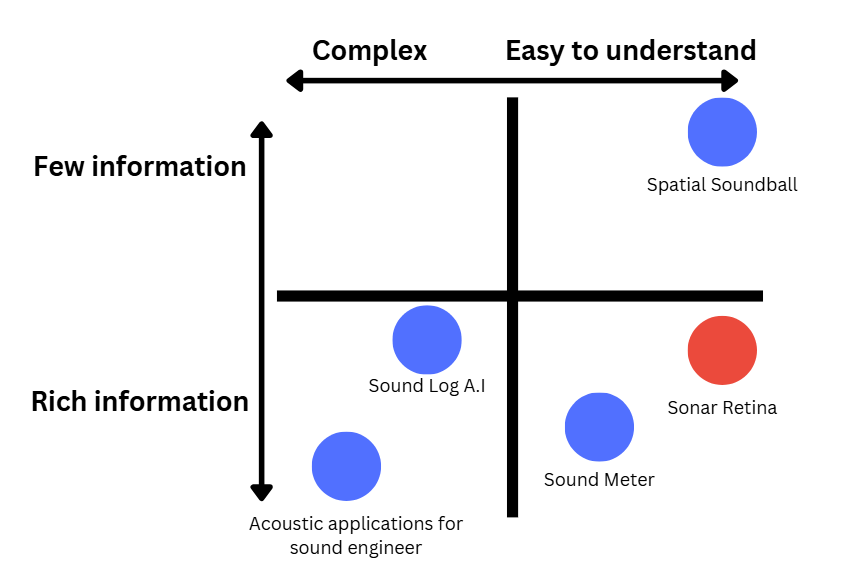
\includegraphics[width=0.8\textwidth]{assets/analysis/asana-analysis.png} 
    \caption{Competitive landscape positioning based on information density and ease of use.}
    \label{fig:positioning-map}
\end{figure}

The competitive landscape for acoustic assistive technology can be categorized into four quadrants based on the relationship between Ease of Use and Information Density.

\begin{itemize}
\item High Information / Low Ease-of-Use (Lower-Left): This quadrant is dominated by professional acoustic engineering tools and data-logging applications such as Sound Log \cite{SoundLog}. 
While these tools provide a high volume of raw data (graphs and logs), their high "Cognitive Load" makes them inaccessible for general users during real-time social interactions.
\item Low Information / High Ease-of-Use (Upper-Left): In contrast, consumer-grade applications like Spatial Sound Ball \cite{SpatialSoundBall} prioritize simplicity and visual aesthetics. 
However, they suffer from "Thin Information," lacking the AI-driven analysis required to identify sound types or specific directional coordinates.
\item Moderate Integration (Lower-Right): Applications such as Sound Meter \cite{SoundMeter} attempt to bridge this gap by providing decibel gauges and basic text-based identification. 
While easier to use than engineering tools, they remain limited in spatial representation.
\end{itemize}

Sonar Retina is strategically positioned in the High Information / High Ease-of-Use quadrant (Upper-Right). Unlike Sound Meter, which sits at the threshold of this category, Sonar Retina moves further along the x-axis by utilizing AI capabilities to automate the "Sound-to-Insight" process. By translating complex directional and semantic data into intuitive icons, the system provides a richer information stream while simultaneously reducing the user's cognitive load.

To evaluate the current state of assistive technology for the deaf and hard-of-hearing, a competitive analysis was conducted using the Asana Competitor Analysis Framework. 
The analysis focused on four core features:

\begin{itemize}
    \item Sound type identification that tells what sound is which Sound Log and Sound Meter have ability to identify.
    \item Sound source distance estimation that tells how far the sound source is which Sound Meter can estimate it from sound volume.
    \item Sound source direction which normally implemented in microphone array of sound engineer applications.
    \item Sound visualization can be various kinds such as sound ball, icon and gauge.
\end{itemize}

As shown in Figure~\ref{fig:positioning-map}, existing solutions often prioritize information rather than visualization to users. 
For instance, \textit{Spatial Sound Ball} \cite{SpatialSoundBall} provides high-quality visualization but lacks the analytical AI to identify sound type, distance and direction. 
On the other hand, \textit{Sound Log} \cite{SoundLog} and \textit{Sound Meter} \cite{SoundMeter} offer robust sound identification and decibel tracking, yet they fail to provide the spatial visualization which is necessary for navigation.

\begin{table}[h]
\centering
\caption{Competitor Analysis of Sound Localization and Visualization Apps}
\label{tab:competitor-comparison}
\begin{tabular}{|l|c|c|c|c|}
\hline
\textbf{App Name} & \textbf{Type} & \textbf{Distance} & \textbf{Direction} & \textbf{Visualization} \\ \hline
Spatial Sound Ball & N & N & N & Ball \\ \hline
Sound Log & Y & N & N & Text \\ \hline
Sound Meter & Y & Y & N & Gauge and text \\ \hline
\textbf{Sonar Retina (Proposed)} & \textbf{Y} & \textbf{Y} & \textbf{Y} & \textbf{Icon} \\ \hline
\end{tabular}
\end{table}

\textbf{Sonar Retina} differentiates itself by integrating all four components into a single interface. By combining AI-driven sound classification with spatial localization, the proposed system provides a complete sound map for the user. 
This holistic approach addresses the primary limitation of current competitors: the inability to provide both "what" and "where" in a simple navigable visual format.

\section{Literature Review}
\label{section:literature-review}

The technical foundation of this project rests on three critical pillars: Sound Source Localization (SSL), Sound Event Detection (SED), and Human-Computer Interaction (HCI) tailored for the deaf and hard-of-hearing community.

\subsection{SSL on Mobile Hardware}
\label{subsec:ssl}
The first technical pillar of this project is the precise localization of sound events. 
According to the systematic review by \cite{Liaquat2021}, SSL is a mature field but faces unique challenges when applied to ad-hoc microphone arrays such as those found in consumer mobile devices. 
The review highlights that while traditional Time Difference of Arrival (TDOA) methods are highly effective, they are sensitive to environmental noise and reverberation—factors that are prevalent in the common settings our application targets.
\\
\\
\textbf{Design Decision:} Building on the comparative analysis provided by Liaquat et al., we chose to implement a robust cross-correlation algorithm (GCC-PHAT). 
This method provides the best balance between computational efficiency for real-time mobile use and the accuracy required to visualize the horizontal direction of sound for the user.

\subsection{SED using Deep Learning}
\label{subsec:sed}
Identifying "what" a sound is requires robust classification. 
We adopt recent advancements in Convolutional Neural Networks (CNNs) optimized for environmental audio. 
According to the work on the AudioSet dataset by \cite{gemmeke2017audio}, pre-trained models like YAMNet provide high-accuracy classification for non-emergency sounds such as laughter, footsteps, and environmental ambience.
A significant challenge in this literature is about polyphonic detection problem, where multiple sounds occur simultaneously.
Moreover, models like YAMNet utilize MobileNetV1 depthwise separable convolutional architecture, which reduces the number of parameters compared to standard CNN models.
\\
\\
\textbf{Design Decision:} We utilize a pre-trained version of the YAMNet model to ensure real-time processing, allowing the app to identify social cues with minimal latency.
We ensure that short duration sounds such as door-knocking, short laugh are captured without being a part of background ambient by using frame-level analysis.
This provides high quality identification required to use in our sound mapping system.

\subsection{Sensory Substitution and Spatial UI Design}
\label{subsec:hci}
A key conceptual framework for this project is the "Sound Bubble" theory proposed by \cite{Eriksson2017}. 
Unlike traditional acoustic management that focuses on noise cancellation or emergency alerts, Eriksson et al. advocate for an "aesthetic additive" approach. 
They define the sound bubble as a micro-space that allows a user to maintain a link with their surrounding activities while filtering for social and sensorial relevance.
This research in HCI for accessibility suggests that "Visual Overload" is a primary reason for abandonment of assistive apps.
If a user is forced to read long text while walking or having a conversation, their "Cognitive Load" increases to unsafe level.
\\
\\
\textbf{Design Decision:} Our UI adopts a "radar-view" approach, prioritizing spatial "texture" and directionality over dense textual logs to reduce cognitive load during interactions.
We try to visualize the sound in radar as icons placed in polar coordinate system to minimize "Time-to-Insight" for users.